\documentclass[
    12pt,
    a4paper,
    titlepage,  % a separate title page
    abstract,  % abstract heading
    headings=standardclasses,  % serif headers
    bibliography=totocnumbered  % references in the TOC
]{scrartcl}
\usepackage[T1]{fontenc}
\usepackage[utf8]{inputenc}
\usepackage[english]{babel}
\usepackage[margin=1in]{geometry}
\usepackage{microtype}

\renewcommand{\baselinestretch}{1.15}
\setlength{\parindent}{0pt}
\setlength{\parskip}{1em}

\setkomafont{author}{\large}  % reduce the font to fit 7 authors on 2 lines
\setkomafont{date}{\large}
\setkomafont{subsubsection}{\fontsize{13pt}{13pt}\selectfont}

% increase abstract header size
\usepackage{etoolbox}
\AtBeginEnvironment{abstract}{\def\sectfont{\large\bfseries}}

% two-level deep TOC
\setcounter{tocdepth}{2}

\usepackage{hyperref}
\hypersetup{
    colorlinks=true,
    linkcolor=black,
    citecolor=black,
    urlcolor=blue,
    pdftitle={NBA Conference Bias}
    }

\usepackage{graphicx}
\graphicspath{ {img/} }

\usepackage{wrapfig}
\usepackage[justification=centering]{caption}  % centered multiline figure caption

\usepackage[lighttt]{lmodern}
\usepackage{amsmath}

\usepackage{longtable}
\usepackage{array}
% aligned table columns of fixed width
\newcolumntype{L}[1]{>{\raggedright\let\newline\\\arraybackslash\hspace{0pt}}m{#1}}
\newcolumntype{C}[1]{>{\centering\let\newline\\\arraybackslash\hspace{0pt}}m{#1}}
\newcolumntype{R}[1]{>{\raggedleft\let\newline\\\arraybackslash\hspace{0pt}}m{#1}}

% a bold italic shortcut
\DeclareTextFontCommand{\textbfsl}{%
  \fontseries\bfdefault % change series without selecting the font yet
  \slshape
}

\usepackage{fancyvrb}
\fvset{baselinestretch=1}

% newfloat prevents additional figure caption spacing
\usepackage[newfloat]{minted}
\setminted{breaklines, linenos}

\title{NBA Conference Bias}
\subject{Harvard University \\ STAT 109 Project}
\author{
    Dmitry Vukolov \and
    Travis Kennison \and
    Kathryn Yates \and
    Jeff Luan \and
    Yingxue Lu \and
    Tyler Stevens \and
    Gbolahan Animashaun
    }
\date{May 2019}

\begin{document}

\maketitle

\begin{abstract}
The National Basketball Association is composed of 30 teams distributed across the United States and equally split between two conferences: the West and the East. We sought to investigate whether there is a potential bias in the NBA that grants teams in one conference a relatively easier path to success due to the differences in travel and schedule. The analysis conducted using a multiple linear regression confirmed the presence of a Western conference advantage, which is consistent with the interconference results observed over the study period. At the same time, the main regression model, constructed with the help of stepwise selection and partial F-tests, showed no significant difference in the effects of travel- and schedule-related factors between the two conferences. Taking into account the weaknesses of the stepwise approach, we applied bootstrap to the variable selection process. The results showed that there is roughly a 65\% chance that the number of time zones crossed during travel might have a different effect on the teams from the two conferences. Additional research would be required to reduce the uncertainty and provide a definitive conclusion.
\end{abstract}

\newpage
\tableofcontents
\newpage

\section{Introduction}
The use of statistics in sports is not a new concept — for generations, avid fans have pored over box scores in the newspaper and marveled over statistical feats like Wilt Chamberlain's 100-point game or Wayne Gretzky's 3,239 career points. However, until fairly recently, what sports fans thought of as ``statistics'' encompassed little more than tally marks; the application of more advanced statistical modeling techniques to sports is still in its infancy, brought into public prominence by the 2003 book \emph{Moneyball}. Since then, more and more professional teams have embraced the power of mathematical and computing methods as they search for competitive advantages in player evaluation, contract negotiation, and game strategy.

The NBA is no different: twenty-nine of the league's thirty teams have at least one staffer dedicated to statistics and analytics\footnote{NBAstuffer, \href{https://www.nbastuffer.com/analytics101/nba-teams-that-have-analytics-department/}{NBA Teams That Have Analytics Department}}, with the Philadelphia 76ers tipping the scale at a staggering nine employees and only the New Orleans Pelicans not devoting any resources to statistical work. These staffers look to tease out any possible source of additional wins for their team; however, we sought to determine whether certain teams are at an inherent advantage or disadvantage to begin with, solely based on their geographic location.

\begin{figure}[ht]
    \centering
    
\includegraphics[width=\linewidth]{nba-map}
    \caption{Location of NBA Teams}
    \label{fig:nba-map}
\end{figure}

Mimicking the distribution of major North American cities, there is a dense cluster of NBA teams in the northeast, mid-Atlantic, and upper Midwest, while the Western teams are far more isolated geographically, even from their within-conference peers\footnote{Image source: Google Images, original author of the map unknown}, see \autoref{fig:nba-map}. As the detrimental effects of extensive travel, particularly across time zones, on athletic performance have been well-documented, we sought to investigate \emph{whether there is potentially a bias in the NBA that allows teams in the Eastern or Western Conferences a relatively easier path to success} due to the differences in travel between the two. Tightly linked to travel are the questions of the NBA schedule, which defines the sequence of trips as well as rest periods for each particular team. Our motivation for investigating this question was its utmost practical importance. Identification of a bias in favor of one of the conferences could initiate additional research and lead to specific actions on the part of either the NBA or the professional teams to eliminate that advantage. Deliberate data-based decisions could be made to equalize the conditions of competitive events during the regular season. Alternatively, a deeper understanding of the effects of those external factors on performance could allow the teams to take extra measures to compensate for their negative effects or use the unfavorable position of the opponent to one's tactical advantage. To our knowledge, no formal research of this particular question has been conducted so far, which further stresses the importance of applying statistical tools to the analysis of potential sources of imbalance between the conferences.

\section{Hypotheses}
The goal of the analysis is to investigate whether there is a ``bias'' in the NBA that allows the Eastern or Western Conferences a relatively easier path to success. To answer this question, we will explore whether the number of miles and/or time zones traveled from game to game has a detrimental effect on performance, and whether that effect is significantly different for one conference versus the other.

Our underlying hypothesis is that \emph{travel does indeed have a negative effect on team performance, particularly as the number of time zones crossed to reach a destination increases}. While we expect to see a statistically significant effect on performance, it should not be a strong indicator of success, as performance metrics that describe the relative strength of teams and their rosters should do a better job of explaining game-level outcomes. Using \emph{p}-values as a measure of strength of evidence, we expect the travel-related indicators to be relatively weak compared to performance-based metrics.

Given that we anticipate a relatively modest (albeit significant) relationship between travel and team-level performance, we do not expect to see a strong difference in travel effects from one conference to the next.

\section{Methods}
\subsection{Data Collection}

A new dataset tailored to answering our research question has been purposefully constructed. It needed to combine the historical data on NBA games on the one hand, as well as the information regarding the itineraries of the teams on the other hand. The data were obtained from two primary sources:

\begin{itemize}
    \item Basketball Reference, an established resource for the NBA statistics
    \item And Google Maps APIs for the location- and travel-related data
\end{itemize}

Basketball is a game with clearly defined rules, highly professional teams, and is widely considered to be a sport where the skill of its players defines the outcome of the game to a much larger degree than do luck or other external factors \cite{mauboussin}. Still, to get a better understanding of the processes and patterns present in the NBA, we chose to look at a period of 18.5 years, spanning from October 2000 till April 2019, thus covering 19 regular NBA seasons — including one season shortened by a bargaining lockout — and 18 completed playoffs. The reasoning behind this decision was that in order to establish the effect of the secondary and presumably weak factors such as travel on player performance, we need a larger sample size. We also anticipated the need to filter the data to be able to focus on the differences between the NBA conferences, which would further reduce its size.

Several web scrapers have been written from scratch to collect the required raw data:

\begin{itemize}
    \item From Basketball Reference on:
    \begin{itemize}
        \item The past NBA games, their schedule and outcome, as well as the resulting team performance
        \item All-NBA awards for the best individual players as a reflection of their strength
        \item The names of the venues where each basketball game took place
        \item The home arenas for the teams in each year, that served as the starting point for traveling at the beginning of the respective season
    \end{itemize}
    \item Using multiple Google Maps APIs:
    \begin{itemize}
        \item To geocode the venues into an exact address and its geographic coordinates (latitude and longitude)
        \item To identify the time zones associated with each geographical location
    \end{itemize}
\end{itemize}

The resulting dataset contained the information on a total of 24,462 games, 8,535 of which took place between one Western and one Eastern Conference team.

\subsection{Data Preprocessing}

Based on the data obtained, an itinerary for every team for the past 18 years has been recreated. As the example in \autoref{fig:bc-itinerary} illustrates, the amount of travel each team undertakes is enormous.

\begin{figure}[ht]
    \centering
    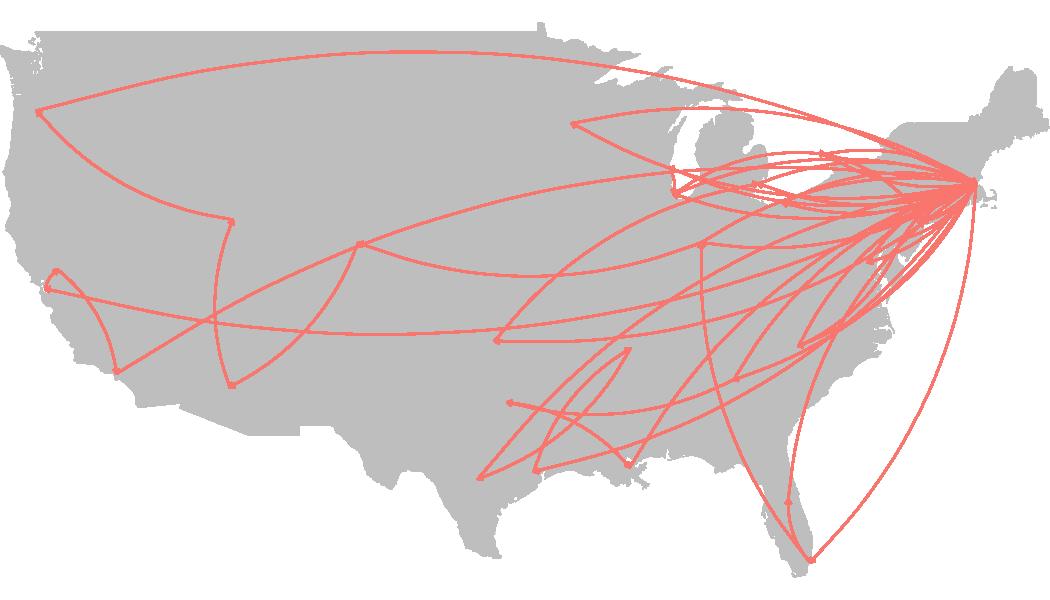
\includegraphics[width=0.95\linewidth]{bc-itinerary}
    \caption{Boston Celtics Itinerary for the 2018-19 Season}
    \label{fig:bc-itinerary}
\end{figure}

The distance each team had to travel has been established in two ways. First, the geodesic distance, which is the shortest distance on the surface of the Earth model has been computed. For that purpose, we used an existing implementation of the algorithm that follows the method described by~\cite{karney}. Secondly, a driving distance for each pairwise combination of the origin and the destination has been acquired via the Google Maps Distance Matrix API. In addition to the distance metrics, we calculated the number of time zones traveled by each team and the direction of travel, eastward vs westward, expressed through the change in the longitude. These basic indicators reflect the amount of travel by each team to a particular location.

To account for the cumulative fatigue associated with constantly being on the road, we chose to compute a set of rolling averages summarizing the amount of travel in a period preceding each event, our line of thought being that a team's performance might depend not only on the number of miles traveled to the most recent event, but also on the amount of travel it had undertaken during the previous week or month.

We also take into consideration several aspects tightly interlinked with travel, which can contribute to a build-up of fatigue. These are the number of days of rest a team had prior to the game, the number of games a team had to play in a fixed period of time and the number of games they played while being on the road. Even though it may seem that a team that has to travel to a game is at a disadvantage compared to a team playing a second consecutive game in one location, this is not actually the case. The second of back-to-back games leave teams with no time to rest, and hence are often discussed as a source of major potential disadvantage.

In order for us to quantify the conference advantage, if any, and also to assess the effect of the weak travel- and schedule-related factors, we need to control for the strongest predictors of team success. The statistical community has developed myriad metrics that attempt to capture the relative strengths of the teams as well as their players. In our analysis we decided to focus on three major groups of performance indicators:

\begin{itemize}
    \item A set of commonly used team performance metrics: the so-called Four Factors, a couple of advanced box score statistics, and the total number of wins for the previous season
    \item Several proxies for the relative team strength based on the number of players with all-NBA awards that actually participated in each particular game
    \item And a manually computed Pythagorean expectation, that is the predicted number of total wins based on the number of points won and lost during the previous season\footnote{Wikipedia, \href{https://en.wikipedia.org/wiki/Pythagorean_expectation\#Theoretical_explanation}{Pythagorean expectation: Theoretical Explanation}}:
    \[
        Pythagorean\ expectation = \frac{points\ for^{14.0}}{points\ for^{14.0} + points\ against^{14.0}}
    \]
\end{itemize}

All of the data mentioned above has been summarized with rolling average indicators and combined in a single dataset for further analysis. The full description of the data is presented in the \hyperref[definitions]{Appendix~\ref*{definitions}}.

\subsection{Statistical Tools}

Our main statistical instrument of choice will be the multiple linear regression for its simplicity and interpretability. In order to accommodate for the regression setting we need to come up with a meaningful response variable and a set of associated predictors.

Each NBA game is represented by the statistics for the two competing teams. Some of the metrics for the two teams are therefore mirrored images of one another: if one team wins, another loses; if one team is the home team, the other is the road team, and so on. A possible solution is to consider the point differential as our response variable (the number of points scored by one team minus the number of points scored by the opponent). Using the point differential as the outcome would allow us to measure the degree of victory of one team over the other. The same reasoning is appropriate for the explanatory variables: it makes perfect sense to regress on the differences between the indicators for the two competing teams. By incorporating the relative metrics rather than the absolute values of the statistics for each team we can correctly model the games where both teams are strong performers or, equivalently, both are weak performers. 

How do we calculate the differentials for each game? Which team should be the baseline and which the opponent? Several research papers dealing with statistical analysis of competitive events have suggested a randomization approach to this problem \cite{carmichael, leard, carr}. Following the recommendation of the authors, for each game we randomly assign one team to be the ``observed'' team, and its opponent the ``baseline''. Random assignment allows us to create two independent groups, making sure that any differences between and within the groups are not systematic. For regression purposes we also limit the dataset to contain just the inter-conference games that are of primary interest to us. This approach also enables us to incorporate a dummy variable corresponding to the conference of the observed team into the regression and measure any bias that may be associated with it.

We test the validity of our random assignment procedure using a set of statistical tests for the mean and the proportion. Their results confirm:

\begin{itemize}
    \item Equal distribution of the conferences within the observed and the baseline groups
    \item The average point differential between the groups that is not significantly different from zero
    \item And the 95\% confidence interval for the proportion of wins that includes 50\%
\end{itemize}

The output of these tests is presented in the \hyperref[random-assign]{Appendix~\ref*{random-assign}}.

The NBA data is inherently a time series collected for a period of more than 18 years. Given a large number of computed predictor variables that try to summarize the time series, we will also employ the stepwise procedure to help us construct a parsimonious and easily interpretable model.  The stepwise method is far from perfect, heavily influenced by the choice of its parameters (``forward'', ``backward'', and other algorithms), as well as by the supplied set of covariates. To gain more confidence in our conclusions we will turn to resampling methods such as bootstrap. Our goal here would be not to evaluate model performance but rather to assess the frequency of inclusion of certain predictors of interest in the final model. The consistent inclusion of a variable into the model and a low \emph{p}-value on bootstrap would reduce the probability of spurious significance. 

\section{Assumptions}

In the course of our analysis, we make several assumptions concerning the data and the employed statistical methods. First, when constructing an itinerary we assume that each team starts at their home arena and, as the season progresses, makes only the trips necessary to get to the next venue according to the NBA schedule. We also assume that if a team has several games in a row in the same city, it stays in that city. We know that these assumptions are not necessarily correct. During the NBA all-star break game in February of each year, the teams may very well return to their home base. Nonetheless, we try to keep our modeling methodology simple, hoping that any omissions in the itinerary are minor and have an equal effect on the Eastern and the Western Conferences.

Secondly, we use the distance between the venues and the difference in time zones as a proxy for the total amount of travel and the resulting fatigue of a team. There may be other factors at play here that we are not taking into account, such as the effect of the mode of transportation, the distance from the venue to the airport, possible unpredicted delays on a trip, and so forth. Since such information is difficult to obtain or outright nonexistent, we stick to the basic available indicators. We also presume that the teams drive to the game if the distance to the next destination is less than 200 miles, and fly otherwise. In the first case, the distance traveled is set to be equal to the driving distance according to Google Maps. In the case of flying, the direct geodesic distance is used as a proxy for the team's fatigue.

Our usage of the built-in \texttt{step()} routine in R for the purposes of model building assumes that the resulting model does not miss any significant predictors. This particular function utilizes the AIC criterion for variable selection, not the \emph{p}-values. It is usually the case that the backward selection method includes all of the significant predictors and many more that may be non-significant. There is, however, no guarantee that it is always so. We try to alleviate this potential issue by manually constructing the models where possible, and by assessing variable importance on bootstrap when it is not. An alternative approach would be to code the stepwise procedure based on \emph{p}-values from scratch or use an existing library that has that functionality.

Finally, we \emph{do not} expect that assumptions of the linear model that we are about to construct are satisfied. Rather we test that it is the case and the model is valid.

\section{Results}

\subsection{Exploratory Data Analysis}

Let's start by evaluating the outcomes of games involving Eastern versus Western Conference opponents to see if there is any meaningful pattern that suggests there is a meaningful bias in the favor of one conference versus another. Throughout this exploratory analysis, we will focus on regular season games, excluding playoff contests, as this is where the majority of interconference play occurs, aside from the NBA finals.

Over the past two decades, the Western Conference has consistently outperformed the East in regular season play. Starting in the 2000-01 season, the West has had the higher interconference winning percentage in all but one season, as shown in \autoref{fig:ic-games}. The pattern is most striking within road interconference games, where the East has particularly struggled compared to their Western Conference counterparts.

\begin{figure}[ht]
    \centering
    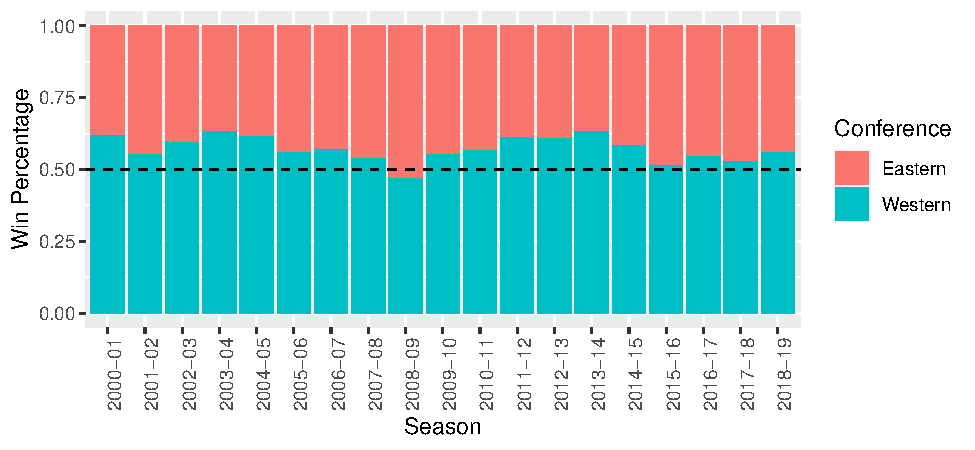
\includegraphics[width=\linewidth]{ic-games}
    \caption{Interconference Regular-Season Games}
    \label{fig:ic-games}
\end{figure}

The dominance of the Western Conference over their Eastern Conference foes is driven by an endless amount of factors, not the least of which is overall team success. In the last 18 seasons, the Western Conference has produced 12 of the last 18 NBA champions. This would suggest that there is an overall talent imbalance in favor of the West.

In the NBA, there is a known phenomenon called ``tanking'', where teams with subpar records attempt to lose on purpose in order to improve their draft positioning. In any given year, it's possible for more ``tanking'' teams to exist in one conference versus the other, which could distort any view of conference superiority based on overall interconference record. To combat this, let's look at the outcome of games across conferences between teams with comparable records.

Let's limit our sample of interconference games to matchups between teams who finished the regular season in the same relative position within their conference. For example, let's look at interconference games between the team with the best record in the East versus the best record in the west; the second-best record in the East versus the second-best record in the west; and so-on. While this is not a perfect control, it should give us a more ``apples-to-apples'' comparison of if and where one conference is consistently outperforming the other.

\autoref{fig:ic-hth} is an 18-year summary of interconference regular season games between comparable seeds from the 2000-01 through 2018-19 regular season.

\begin{figure}[ht]
    \centering
    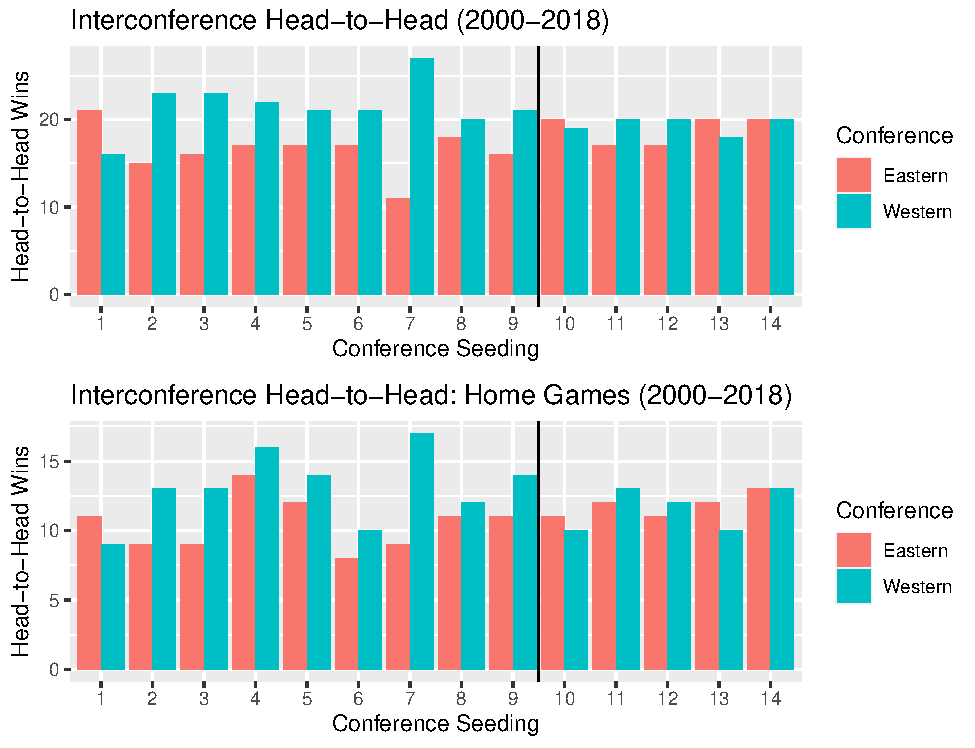
\includegraphics[width=\linewidth]{ic-hth}
    \caption{Interconference Head-to-Head Games}
    \label{fig:ic-hth}
\end{figure}

From this view, we can see that Western Conference teams have owned the head-to-head matchups versus the East within seeds 2-through-9, which almost exactly equates to the NBA playoff format (seeded 1-through-8). From this standpoint, the West has clearly been the dominant conference among playoff eligible teams for the past 18 seasons. There has, however, been more parity between the number one seeded teams, which makes some sense given that the East has crowned six NBA champions since 2000.

Another way to evaluate relative performance of one conference versus another is using point differential. Point differential is defined as the difference between points scored and points allowed, where a positive number reflects a winning outcome and negative point differential indicates a losing outcome. This metric is beneficial for use in regression analysis for several reasons:

\begin{enumerate}
    \item It is a continuous variable well-suited for linear regression
    \item It can measure the impact of winning and losing as well as extreme outcomes
    \item Differences often eliminate serial correlation within the data
    \item It is easy to interpret (positive equals to a win, negative to a loss)
\end{enumerate}

As we can see from \autoref{fig:point-diff}, the point differential for the Western Conference versus the Eastern Conference exhibits the same pattern of Western dominance. Within interconference regular season games, the West won the combined point differential battle in 17 of the last 18 seasons (excluding 2008-09 which had only 66 regular season games). However, the Western Conference point-differential has declined since its peak in 2013-14, as Eastern Conference teams have become more competitive, particularly on the road. The pattern is almost sinusoidal which begs the question of whether this is a cyclical pattern.

\begin{figure}[ht]
    \centering
    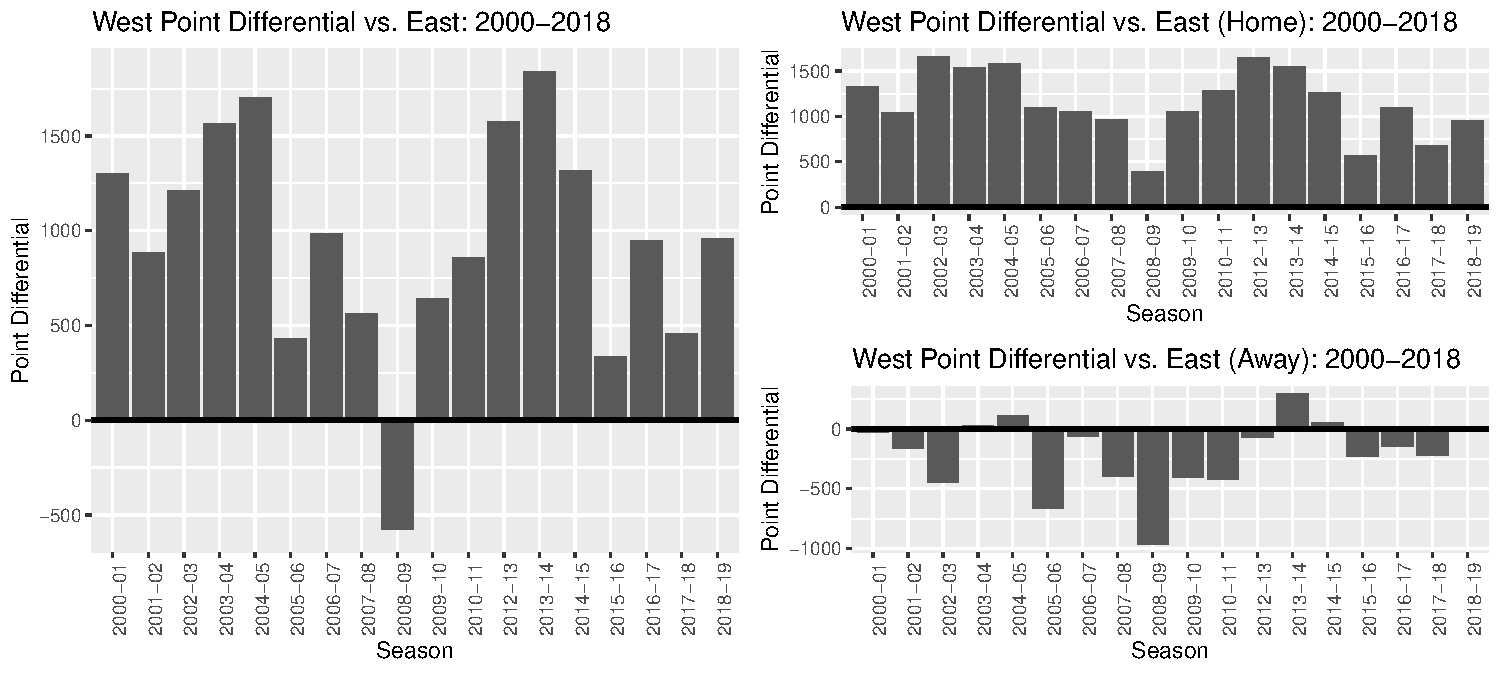
\includegraphics[width=\linewidth]{point-diff}
    \caption{Interconference Point Differential}
    \label{fig:point-diff}
\end{figure}

The map in \autoref{fig:home-areans} depicts the home arena locations for all 30 NBA teams, and the 8 franchises that have won the NBA title since the turn of the century (in gold). The locations of these title-winning franchises are scattered along the periphery of the U.S. border. Along with possessing superior talent, it's fair to ask whether these franchises have benefited from their geographical locations. Does the amount of travel required to reach these locations have a negative effect on their opponents performance?

\begin{figure}[ht]
    \centering
    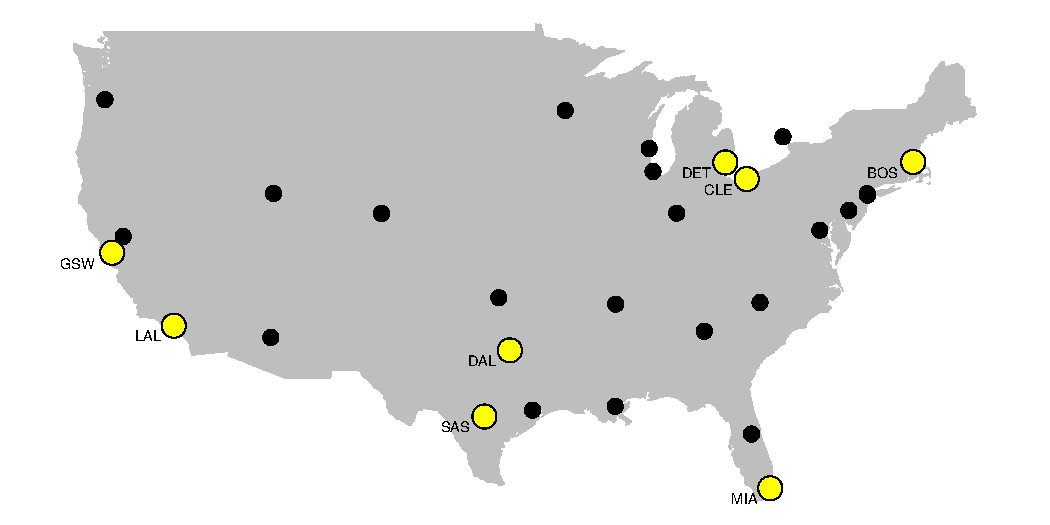
\includegraphics[trim=10 10 20 10,clip,width=\linewidth]{home-arenas}
    \caption{Home Arena Locations for All 30 NBA Teams \\ (NYC and LA With Two Teams Each)}
    \label{fig:home-areans}
\end{figure}

\subsubsection*{Travel by Conference}

In order to answer the question posed above, let's examine the amount of travel undertaken by each team over the course of a season, and over the course of several seasons. \autoref{fig:dist-total} shows the \emph{total distance traveled} for each team during the 2017-18 regular season. We can see that overall distance traveled is generally higher when comparing East vs. West in ascending order of total travel distance (left-to-right).

\begin{figure}[ht]
    \centering
    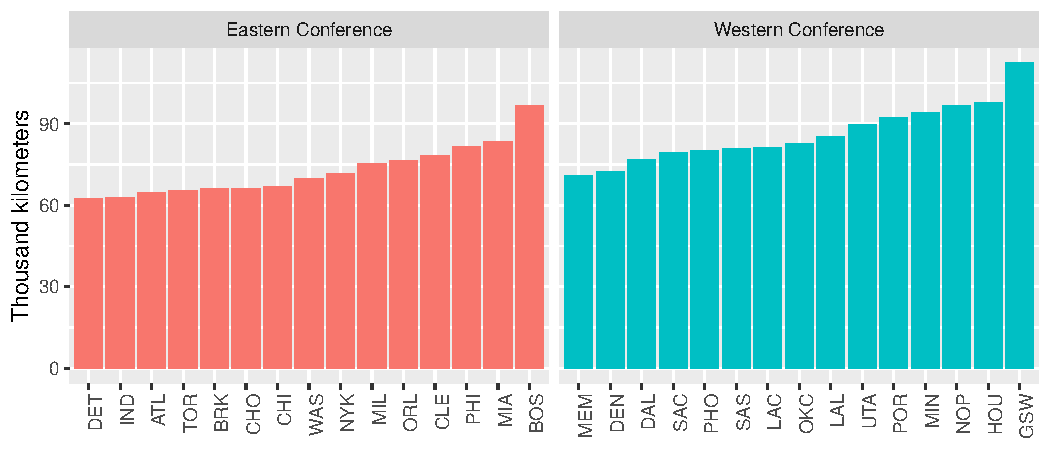
\includegraphics[width=\linewidth]{dist-total}
    \caption{Total Distance Traveled During the 2017-18 Season}
    \label{fig:dist-total}
\end{figure}

\autoref{fig:dist-distrib} illustrates the \emph{distribution of total distance traveled} for each team during the same timeframe (2017-18 regular season). The height of the boxplots on the right are higher than those on the left, indicating that Western Conference teams take more frequent long-distance trips than the East. However, while Eastern Conference teams take fewer long-distance trips, the trips they do take are much longer by comparison, as illustrated by the outliers on the left.

\begin{figure}[ht]
    \centering
    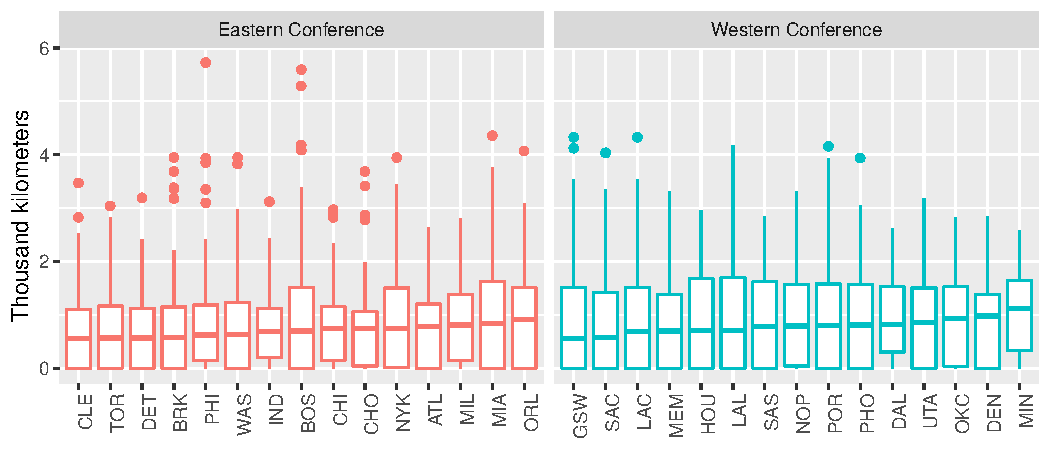
\includegraphics[width=\linewidth]{dist-distrib}
    \caption{Distribution of Distance Traveled During the 2017-18 Season}
    \label{fig:dist-distrib}
\end{figure}

When regressing total distance traveled on a conference indicator variable (equivalent to a two-sample t-test), we conclude that Western Conference teams traveled more than Eastern Conference teams in the 2017-18 season (see full code in the \hyperref[travel-test]{Appendix~\ref*{travel-test}}).

\begin{Verbatim}
> summary(lm(formula = total_dist_traveled ~ conference,
             data = cumulative_travel))

Coefficients:
            Estimate Std. Error t value Pr(>|t|)    
(Intercept)    72569       2665  27.229  < 2e-16 ***
conferenceW    13680       3769   3.629  0.00112 ** 
---
Signif. codes:  0 ‘***’ 0.001 ‘**’ 0.01 ‘*’ 0.05 ‘.’ 0.1 ‘ ’ 1

Residual standard error: 10320 on 28 degrees of freedom
Multiple R-squared:  0.3199,    Adjusted R-squared:  0.2956 
F-statistic: 13.17 on 1 and 28 DF,  p-value: 0.001124
\end{Verbatim}

This conclusion also holds when looking at distance traveled by conference over the last 18 regular seasons. \autoref{fig:dist-conf} shows that Western Conference teams consistently travel more than Eastern Conference teams on a year-to-year basis.

\begin{figure}[ht]
    \centering
    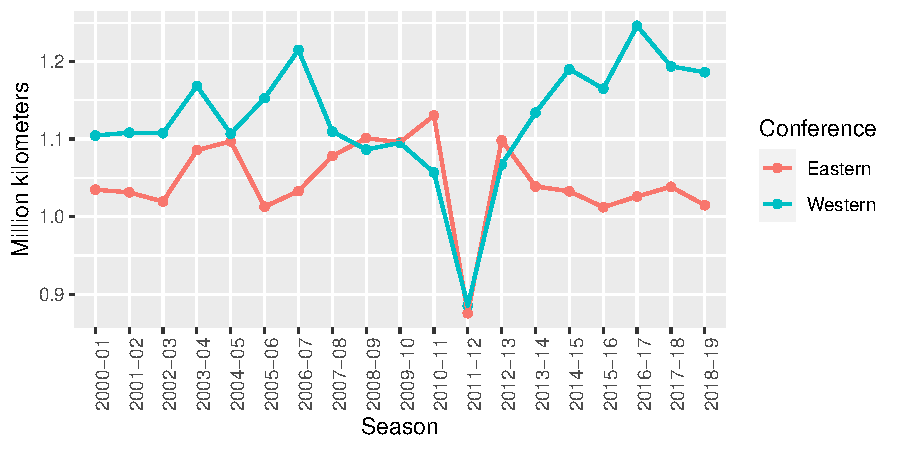
\includegraphics[width=\linewidth]{dist-conf}
    \caption{Total Distance Traveled by Conference}
    \label{fig:dist-conf}
\end{figure}

\subsubsection*{Interconference Games}

While the West does travel more than the East over a full regular season, the travel distance between conferences is much closer within interconference games, see \autoref{fig:dist-ic}. This makes sense in practice, as these teams are traveling to each other once a year, so the travel distance should largely cancel each other out.

\begin{figure}[ht]
    \centering
    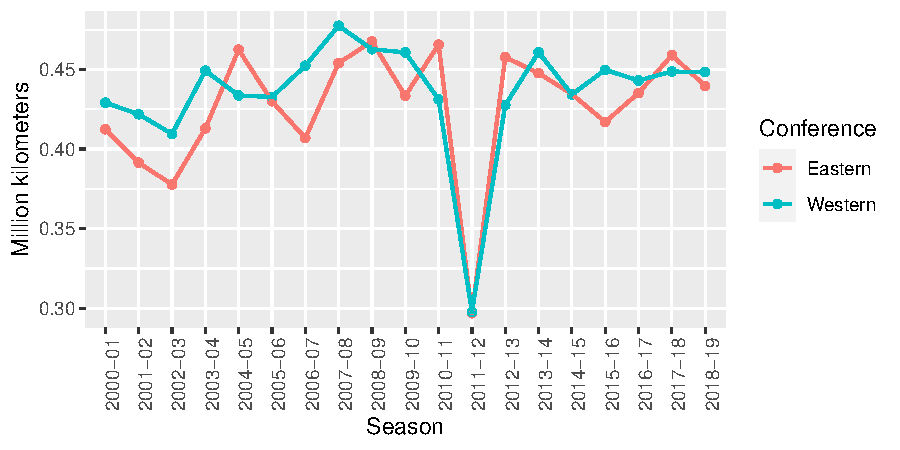
\includegraphics[width=\linewidth]{dist-ic}
    \caption{Interconference Distance Traveled by Conference}
    \label{fig:dist-ic}
\end{figure}

However, while the distance traveled to get to an interconference game may be the same, the total distance traveled over a 3-day and 7-day period is not the same across conferences. When playing an interconference game, the Western Conference consistently travels more than the Eastern Conference over a 3-day and 7-day period, as evidenced by \autoref{fig:dist-ic-days}.

\begin{figure}[ht]
    \centering
    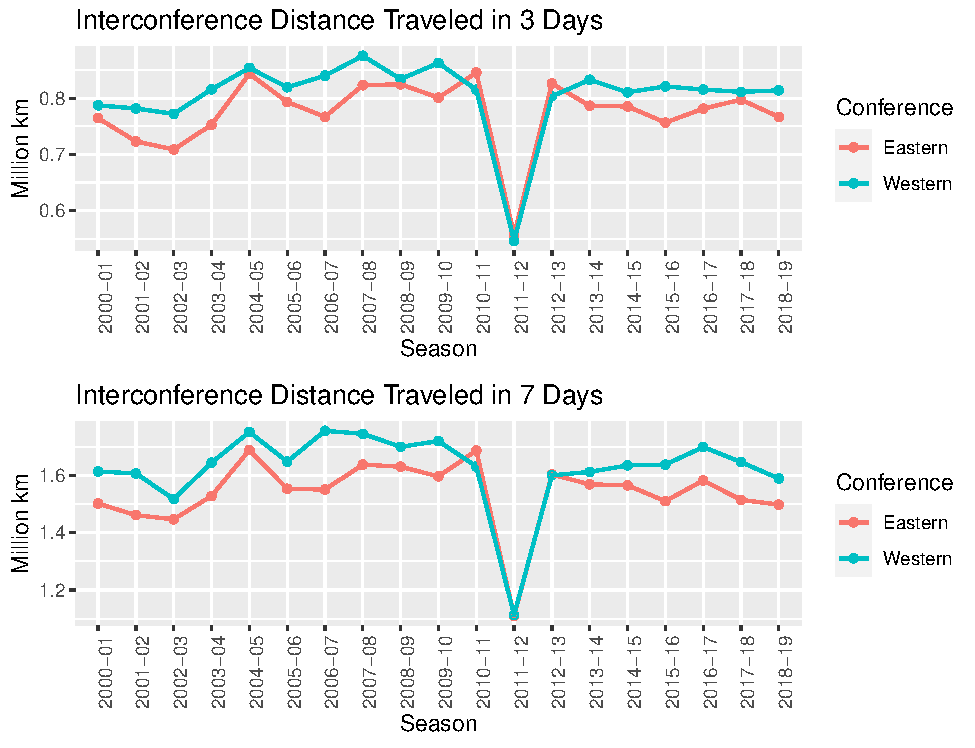
\includegraphics[width=\linewidth]{dist-ic-days}
    \caption{Interconference Distance Traveled Over 3 and 7 Days}
    \label{fig:dist-ic-days}
\end{figure}

\subsection{Model Building}

To quantify the potential conference advantage we build two models:

\begin{enumerate}
    \item The basic model with a conference dummy variable that controls for the relative strength of each conference.
    \item The expanded model that evaluates the effects of travel- and schedule-related factors and their interactions with the conference dummy. This model contains only the predictors that are significantly associated with the response at the 0.05 significance level.
\end{enumerate}

We construct the first model by regressing the point differential on a dummy variable for the conference and all available team performance indicators (the results are presented in the \hyperref[model1]{Appendix~\ref*{model1}}). Since many of the coefficients in the resulting model are not significantly different from zero, we manually build a reduced model containing only the predictors correlated with the outcome. A partial F-test confirms that we can indeed drop all of the non-significant predictors at once ($p\operatorname{-value} = 0.52 > 0.05$). When controlling for the most basic predictors of team performance the Western Conference still demonstrates an advantage: the point differential for the teams in this conference is higher \emph{on average} by almost 2 points than for the teams from the Eastern Conference:

\begingroup
    \ttfamily
    \begin{longtable}{|l|r|r|r|r|}
        \hline
        \textbf{term} & \textbf{estimate} & \textbf{std\_error} & \textbf{statistic} & \textbf{p\_value} \\ \hline
        \endhead
        intercept & -1.09 & 0.195 & -5.589 & 0 \\ \hline
        conferenceW & 1.997 & 0.284 & 7.025 & 0 \\ \hline
        total\_wins\_ly & 0.021 & 0.008 & 2.618 & 0.009 \\ \hline
        pyth\_40games & 21.419 & 0.906 & 23.646 & 0 \\ \hline
        tpar\_40games & 6.268 & 2.3 & 2.725 & 0.006 \\ \hline
        steal\_40games & 0.229 & 0.11 & 2.075 & 0.038 \\ \hline
        drb\_40games & 0.111 & 0.056 & 1.983 & 0.047 \\ \hline
    \end{longtable}
\endgroup

This is consistent with what we've observed during the exploratory data analysis. The Western Conference has been dominating the Eastern Conference in the inter-conference games for the past two decades.

We then proceed to build an expanded model (\hyperref[model2]{Appendix~\ref*{model2}}). To understand whether there is an effect of the presumably weak travel- and schedule-related factors we add those to the full regression model. We also incorporate the interaction terms between the conference dummy and the aforementioned proxies for team fatigue. All of the predictors and the response demonstrate normal-like distribution and do not require any transformations for reasons that we will show during diagnostics, so we add them to the model as is. There are in total 137 explanatory variables in the full model, which is very large. With the help of the stepwise procedure and a backward-forward selection method we are able to reduce the number of predictors to 28. Some of them are not significant, while our goal is to obtain a model best suited for inference that is possible to interpret. Therefore we continue to trim the model manually by means of a partial F-test, further reducing the number of covariates. Additionally, we check the variance inflation factors, drop the predictors with the highest values and continue to manually remove any explanatory variable whose \emph{p}-value is above 0.05 \emph{one at a time}. We end up with a model containing 19 predictor variables, including one interaction term, all of which are significantly associated with the response at the 5\% significance level:

\begingroup
    \ttfamily
    \begin{longtable}{|l|r|r|r|r|}
        \hline
        \textbf{term} & \textbf{estimate} & \textbf{std\_error} & \textbf{statistic} & \textbf{p\_value} \\ \hline
        \endhead
        intercept & -6.1978 & 1.3912 & -4.4549 & 0 \\ \hline
        date & 0.0002 & 0.0001 & 2.1402 & 0.0324 \\ \hline
        home\_team & 5.1983 & 0.3802 & 13.6739 & 0 \\ \hline
        conferenceW & 5.1013 & 1.9946 & 2.5576 & 0.0106 \\ \hline
        dist\_3days & 0.0003 & 0.0001 & 2.3783 & 0.0174 \\ \hline
        same\_tz\_3days & -0.5583 & 0.2284 & -2.444 & 0.0145 \\ \hline
        tz\_total\_3days & -0.8756 & 0.2216 & -3.9522 & 0.0001 \\ \hline
        tz\_total\_30days & 0.1096 & 0.0356 & 3.074 & 0.0021 \\ \hline
        days\_rest & -0.551 & 0.169 & -3.2606 & 0.0011 \\ \hline
        second\_backtoback & -1.8416 & 0.335 & -5.4968 & 0 \\ \hline
        road\_7days & -0.2535 & 0.1041 & -2.4345 & 0.0149 \\ \hline
        pyth\_40games & 19.7425 & 0.8162 & 24.1885 & 0 \\ \hline
        tpar\_40games & 6.7834 & 2.3682 & 2.8644 & 0.0042 \\ \hline
        steal\_40games & 0.3077 & 0.1083 & 2.8417 & 0.0045 \\ \hline
        orb\_40games & 0.0809 & 0.0388 & 2.0868 & 0.0369 \\ \hline
        drb\_40games & 0.1184 & 0.0547 & 2.1667 & 0.0303 \\ \hline
        first\_team\_nba\_ly & 1.7415 & 0.2728 & 6.3835 & 0 \\ \hline
        second\_team\_nba\_ly & 1.4616 & 0.2721 & 5.3709 & 0 \\ \hline
        third\_team\_nba\_ly & 1.1193 & 0.2694 & 4.1543 & 0 \\ \hline
        date:conferenceW & -0.0003 & 0.0001 & -2.0197 & 0.0434 \\ \hline
    \end{longtable}
\endgroup

All of the regression terms can be grouped into several categories:

\begin{itemize}
    \item \textbf{Conference advantage:} we detect a significant difference between the expected point differential for the two conferences. For the Western Conference teams the differential is on average 5.1 points higher than that for the Eastern Conference teams, all other variables held constant.
    \item \textbf{Time:} which includes the date expressed in days and its interaction term with the conference. The average point differential for the Eastern Conference teams has been increasing over the decades, in contrast to the Western Conference teams, whose net point differential is negative. Therefore, the gap between the conferences has been decreasing over time, albeit by a very small margin.
    \item \textbf{Home advantage:} there is a highly significant difference between the expected point differential for the home team and the road team. A team playing at home is at a distinct advantage whose effect is comparable to the conference advantage and may either entirely offset it, or amplify it. Holding all other variables fixed, the expected point differential for Western Conference teams shrinks from $4.1$ to $-1.1$ points (on average) when playing at home versus on the road, so home court advantage is indeed a significant factor.
    \item \textbf{Travel-related indicators:} include the distance traveled for the past three days, the number of games played in the same time zone and the amount of travel across time zones. These need to be interpreted while holding every other predictor variable fixed and may not be very meaningful on their own. Importantly, no interactions are deemed significant, so the effect of travel is the same for the two conferences.
    \item \textbf{Schedule-related predictors:} including the number of days of rest, the indicator for the second of back-to-back games and the number of road games. Playing two games in a row with no rest is a highly significant predictor which has a negative impact on the expected point differential. Here again, no interactions made their way into the final regression model, so the impact of schedule is approximately the same for the teams from both conferences.
    \item And finally the \textbf{relative team strength} statistics, which we control for: as these go up for the observed team or go down for the opponent, the degree of victory is expected to be higher on average, which makes perfect sense.
\end{itemize}

Note that all of the above relationships refer to an \emph{association} between the predictors and the outcome. The data were collected retrospectively and serve as the basis for an observational study. This is not an experiment, and no causal statements can be made.

To get an initial understanding of model stability, we also implement an alternative approach to constructing the final model. In it, we first build a model using stepwise, trim it based on a partial F-test to contain just the significant predictors, and only then add interactions with the conference to the model. The resulting regression produces similar results, though some of the variables that are significant in our main model do not make their way into the alternative model. These are the predictors with relatively higher \emph{p}-values: the date and its interaction term, the distance traveled for the past three days and the number of road games played during the previous week. All other explanatory variables remain in the model and support our main conclusions.

\subsection{Diagnostics}

To ensure that our conclusions are valid, we perform model diagnostics and see if the assumptions of linear regression are satisfied, see \autoref{fig:diag} and \hyperref[diag-code]{Appendix~\ref*{diag-code}}. Let us go through the assumptions one by one.

\begin{figure}[ht]
    \centering
    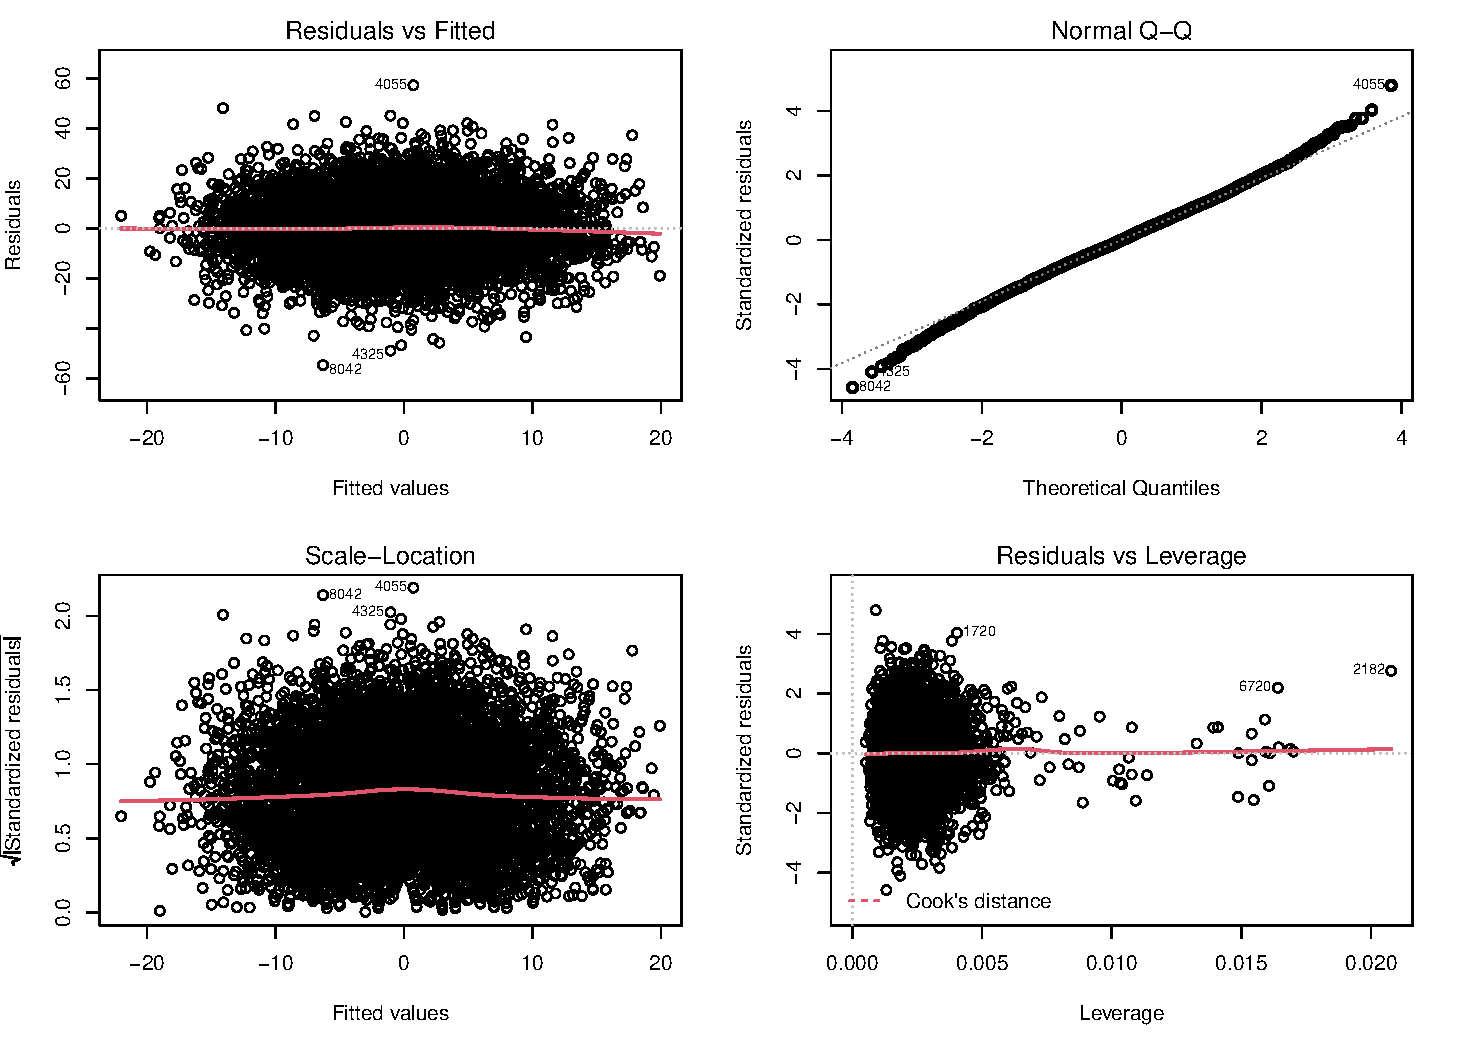
\includegraphics[width=\linewidth]{diag}
    \caption{Checking the Assumptions of Linear Regression}
    \label{fig:diag}
\end{figure}

\textbf{Linearity:} The relationship between the residuals and the fitted values is linear: the residuals are randomly scattered around the zero line and the LOWESS smoother presents a straight line. Many observations have high standardized residuals, much larger than 2.0 in absolute value. These seem to have little influence on the resulting regression line, as evidenced by the Residuals vs Leverage plot. A couple of points with relatively high leverage and high residuals do exist, but those are well below the critical value of 0.5 for the Cook's distance. 

\textbf{Normality of errors:} Even though the residuals appear to deviate slightly from the normal Q-Q line, as we mentioned before there are a lot of standardized residuals with absolute values higher than 2.0. A formal test for normality confirms that the residuals are not normally distributed. Here we are using the Anderson-Darling test for normality instead of the Shapiro-Wilk test since the latter is limited to a sample size of 5000. A small \emph{p}-value of 1.982e-05 for the normality test makes us reject the null hypothesis and state that the residuals are not normal. This issue, however, is largely alleviated by a large sample size of our dataset. With 8,535 observations in the regression, we expect the Central Limit Theorem to kick in and result in normally distributed estimates of regression parameters.

\textbf{Constant variance of noise:} The noise is homoskedastic, as demonstrated by the Scale-Location plot. The variance of the residuals is the same across all the fitted values. This is additionally confirmed by a formal Breusch-Pagan test. The obtained \emph{p}-value is 0.557, which leads to failing to reject the null hypothesis of homoskedastic noise.

\textbf{Independence:} Since the data originally collected represent a time series, one cannot assume independence of noise and need to check for that. The run of a Durbin-Watson test for independence outputs a statistic of 2.026 and a \emph{p}-value of 0.238 — the values that are consistent with independence. It may seem counterintuitive how a regression on a time series data is able to demonstrate an almost ideal picture in terms of model diagnostics. The reason behind it is that the data actually regressed is not the original time series, but rather the differences in statistics for the competing teams. This approach turns out to be both a reasonable choice for modeling a competitive event and allows for obtaining a valid and interpretable model.

\textbf{Multicollinearity:} an additional test for multicollinearity is performed by computing the variance inflation factors. All of the values are small except for the VIFs of the terms involved in interactions. These are expected to be high and do not pose an issue\footnote{Paul Allison, \href{https://statisticalhorizons.com/multicollinearity}{When Can You Safely Ignore Multicollinearity?}}. The largest VIF for non-interaction terms is 6.9, which is well below the commonly used threshold of 10 for high amounts of collinearity.

Overall, the model satisfies all of the assumptions of linear regression except for normality of errors, the issue that is mitigated by a large sample size. Such a model is valid and allows for interpretation.

\subsection{Bootstrap}

Our current method for building a regression model out of more than a hundred predictors is based on a combination of a stepwise approach and a set of partial F-tests or, alternatively, iterative elimination of variables using \emph{p}-values one at a time. The stepwise method, in particular, is not without its weaknesses. It does not guarantee the best model or the inclusion of all significant predictors in the model. As an additional way to assess potential variability in the results and the impact that those may have on our conclusions, we turn to resampling tools, namely to bootstrap. By repeatedly drawing random samples of the same size as our dataset, with replacement, bootstrap allows us to evaluate the whole model selection procedure as if we were doing it on the population as a whole.

For that purpose, we wrote a procedure that draws random samples of data, runs the stepwise function, drops any insignificant predictors based on their \emph{p}-values, one at a time in descending order, and records the configuration of the final model that contains only the significant predictors. We used the standard significance level of 0.05 as our threshold. The process was repeated 100 times. The number of bootstrap iterations may be seen as low, which is justified only by computational demands of the stepwise algorithm. Still, it gave us a glimpse into the relative frequencies with which particular predictor variables are selected for inclusion in the model. Our experiments have shown that in our case these numbers are quite stable starting from 50 iterations of the bootstrap procedure. \autoref{fig:bootstrap} summarizes the results with respect to the travel- and schedule-related factors that are of interest to us. We also only show the explanatory variables that were included in the model as significant more than 25\% of the time.

\begin{figure}[ht]
    \centering
    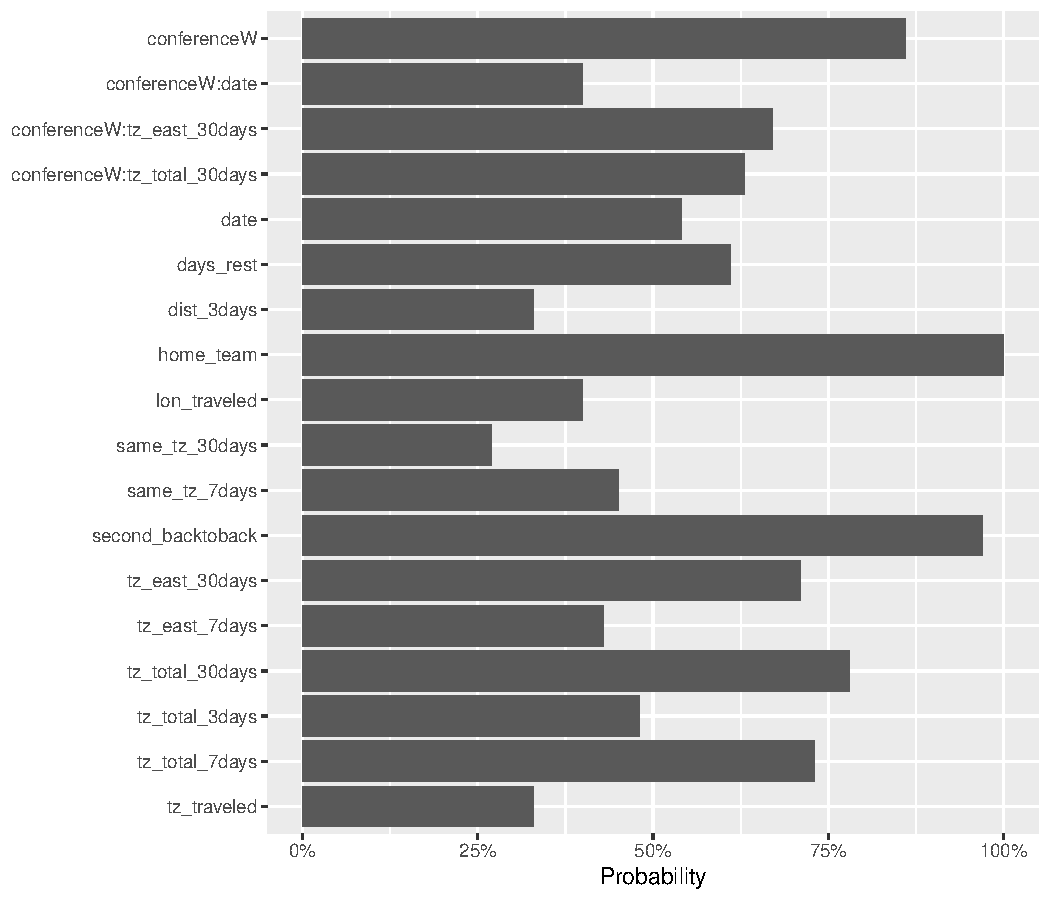
\includegraphics[width=0.9\linewidth]{bootstrap}
    \caption{Predictor Probability of Being Included in the Model}
    \label{fig:bootstrap}
\end{figure}

The procedure informs us of the relative strength of evidence for different schedule and travel indicators. In particular, the home team advantage is significant in 100\% of the models constructed using the employed method. The same can be said about the second of back-to-back games, which is almost as frequently selected for the final model. The advantage (or at the very least a difference) of the Western Conference is also present in 86\% of the cases. Importantly, time zone related factors have a high probability of being chosen as significant. What we did not capture with our original single model was the potential importance of two interaction terms: the number of time zones traveled in total and in the eastward direction specifically during the month preceding the game might have a different effect on the Western Conference compared to the Eastern Conference. These terms are included as statistically significant in the model in roughly 63-67\% of the cases. We believe that it is premature to decisively state that there is a bias in the NBA with respect to these factors in favor of one of the conferences. However, it surely can serve as an indication of the need for further professional research.

\section{Limitations}

Our conclusions regarding the NBA conference advantage on the basis of a regression model agree with the observations from the exploratory data analysis of the past games. Still, the obtained regression model explains only 22\% of the variability in the point differential. This is consistent with the range of $R^2$ values obtained by authors doing similar research, e.g. \cite{carr}. Our attempt to control for the relative team strength made use of multiple performance metrics, both readily available and specially computed by the authors. Yet, the game dynamics are infinitely more complex, and cannot be captured fully by just a handful of indicators. The state of the art methods for predicting team performance are most often built by aggregating the characteristics of individual players, taking into account the time that these players spend in the game, the interactions between the players and their contribution to the team, as well as such aspect as the overall career path of individual players and its similarity to historical comparables\footnote{FiveThirtyEight, \href{https://fivethirtyeight.com/methodology/how-our-nba-predictions-work/}{How Our NBA Predictions Work}}. These efforts are beyond the scope of the current paper. At the same time, we need to acknowledge that the outcome of a regression model would most likely be different if it better accounts for the expected performance of the competitors. While we do not expect our conclusions regarding the presence of the Western Conference advantage to change, its magnitude reflected in the regression estimates most definitely will. It is more difficult to confidently predict whether the relatively weaker travel- and schedule-related factors will still play a significant role when the team performance characteristics are better taken into consideration. Our anticipation is that some of those explanatory variables with particularly high \emph{p}-values like the home advantage, the second of back-to-back games and the number of time zones changed will still be significant, while others like the distance traveled will lose their importance. Further research will need to be conducted to properly assess these aspects.

\section{Challenges}

Sports in and of themselves are inherently unpredictable; the sheer amount of factors that could potentially contribute to player performance is staggering, and many are difficult to quantify, providing the human element that makes the game worth watching and the narratives worth following. The sheer magnitude of information that could potentially be of use was challenging to distill down to the scope of this project. A lot of effort has been put into choosing the most appropriate metrics, writing the code to obtain the raw data from multiple sources, merging the game-level data and season-level, team-level data. We also did our best at converting the available data to a format that could be used to answer our research questions. That meant constructing the itinerary for each team, computing the rolling averages that summarize the time series and finding a way to model competitive events within a linear regression framework. For the sake of brevity, we do not list all the code in the Appendix, but rather make it available upon request.

\section{Conclusions}

\begin{wraptable}{r}{0.42\textwidth}
    \vspace{-12pt}
    \hspace{10pt}
    \small
    \begin{tabular}{|l|R{18mm}|R{18mm}|}
    \hline
        \footnotesize{\textbf{Season}} & \footnotesize{\textbf{Point Diff West-East}} & \footnotesize{\textbf{Point Diff per Game}} \\ \hline
        2000-01 & 1,301 & 3.1 \\ \hline
        2001-02 & 884 & 2.1 \\ \hline
        2002-03 & 1,215 & 2.9 \\ \hline
        2003-04 & 1,568 & 3.7 \\ \hline
        2004-05 & 1,703 & 3.6 \\ \hline
        2005-06 & 429 & 1.0 \\ \hline
        2006-07 & 987 & 2.2 \\ \hline
        2007-08 & 563 & 1.2 \\ \hline
        2008-09 & $-576$ & $-1.2$ \\ \hline
        2009-10 & 644 & 1.4 \\ \hline
        2010-11 & 860 & 1.8 \\ \hline
        2011-12 & 780 & 2.6 \\ \hline
        2012-13 & 1,579 & 3.3 \\ \hline
        2013-14 & 1,841 & 4.1 \\ \hline
        2014-15 & 1,320 & 2.9 \\ \hline
        2015-16 & 336 & 0.7 \\ \hline
        2016-17 & 946 & 2.1 \\ \hline
        2017-18 & 456 & 1.0 \\ \hline
        2018-19 & 958 & 2.1 \\ \hline
        Average & 937 & 2.1 \\ \hline
    \end{tabular}
    \vspace{-12pt}
\end{wraptable}

The exploratory section of the analysis illustrates the clear pattern of Western Conference dominance within interconference play. In 18 of the last 19 regular seasons, Western Conference teams have outscored their Eastern Conference opponents by an average of 2.1 points per-season within head-to-head matchups (see right). We observed the same degree of Western Conference dominance when evaluating the head-to-head results of interconference games between teams with similar records. As we saw earlier, the West has enjoyed an even bigger head-to-head advantage against playoff-eligible teams than against non-playoff teams. This is further illustrated by the fact that the Western Conference has crowned 12 of the past 18 NBA champions.

While the dominance of the Western Conference is likely driven by many factors, particularly roster composition and an overall imbalance of player talent, we wanted to explore whether the detrimental effects of travel are different for Western Conference teams versus Eastern Conference teams, and whether this creates an easier path to success for one conference versus another. 

In the full regression model presented above, there are four \textbf{travel-related} indicators, three \textbf{schedule-related} variables, eight predictors reflective of \textbf{team strength}, and regression terms capturing the effect of \textbf{conference advantage}, \textbf{home-court advantage}, and \textbf{time} (trend).

Using \emph{p}-values as strength of evidence, Pythagorean win expectation has the strongest relationship with point differential, followed by the number of all-NBA player participants, and indicator variables for home games and the second of back-to-back games. After that, the time-zone travel indicators are the next most significant predictors of point differential, which is consistent with our original hypothesis that time zones would be the strongest measure of travel, and would exhibit a negative effect on performance. The other performance-metrics and travel related indicators are significant at the 0.05 level, but they are far less significant than the variables listed above. Overall, this result is consistent with our original hypothesis: the negative effect of travel on team performance is significant, but it is a less relevant predictor of team success compared to team performance metrics that describe the strength of a team's roster.

As mentioned earlier, only one interaction variable, that which represented a combination of the date of each game and the conference of the observed team, was shown to have a statistically significant relationship with team performance. Although, when performing repeated stepwise selection (with replacement) via the bootstrap procedure, we found two additional time zone-related factors that had a statistically significant interaction with the conference dummy variable in roughly 63-67\% of repeated trials. While we know stepwise regression is an imperfect method of model selection, the observed probability of inclusion for these travel-related terms could be a potential source of future analysis.

\section{Further Discussion}

The analysis conducted in the current paper can serve as the basis for subsequent research. Building upon the approach of modeling point differential, one can considerably improve it by expanding the ways in which the time series is summarized. In addition, player-level data can be added to the models to provide the granularity needed and better account for the idiosyncrasies of sports. Our decision was to utilize the most basic set of averages with several choices of rolling windows, which may be insufficient to capture the signal present in the data. By making use of other statistics and other window periods to describe both the strong and the weak factors influencing the outcome of the game, one may get a better insight into the dependencies and patterns present in the NBA. This, coupled with more advanced techniques for evaluating team performance, will add the most value to the analysis conducted so far.  

Additionally, potential sources of conference bias may stem not only from the travel- and schedule-related aspects of an NBA season. Promising directions for further research include investigation of predisposition to injury, and whether teams in one conference lose more man-games to injury than the other conference. Of high practical importance to professional teams are also the questions of attracting superstar players, and whether one conference is inherently more successful at that than the other conference. Moreover, organizational and lifestyle traits which characterize each conference, their adaptability and decision horizon, along with the stability of ownership or lack thereof may all serve as the sources of conference bias. We leave further investigation of such variables to other researchers.

\begin{thebibliography}{Mauboussin 2012}
\bibitem[Albert 2007]{albert} 
Albert, J., Koning, R. (2007). \textsl{Statistical Thinking in Sports (1st ed.)}. CRC Press.

\bibitem[Carmichael 2000]{carmichael}
Carmichael, F., Thomas, D., Ward, R. (2000). \textsl{Team Performance: the Case of English Premiership Football}. Managerial and Decision Economics, 21(1), 31–45.

\bibitem[Carr 2015]{carr}
Carr, J. (2015). \textsl{The Home-Court Advantage Effect in NBA Basketball}. A Thesis Submitted to the Department of Economics of the University of Ottawa.

\bibitem[Carter 2017]{carter}
Carter, K. (2017). \textsl{Relative Home‐Court Advantage: The Impact of Travel on Team Production When One Team is Closer than its Opponent to a Neutral Game Site}. Managerial and Decision Economics, 38(1), 76-91.

\bibitem[Entine 2008]{entine}
Entine, O., Small, D. (2008). \textsl{The Role of Rest in the NBA Home-Court Advantage}. Journal of Quantitative Analysis in Sports, 2008, Volume 4, Issue 2.

\bibitem[Jones 2016]{jones}
Jones, S. (2016). \textsl{Predicting Outcomes of NBA Basketball Games}. A Thesis Submitted to the North Dakota State University, Department of Statistics.

\bibitem[Karney 2013]{karney}
Karney, C. (2013). \textsl{Algorithms for Geodesics}. Journal of Geodesy, 87(1), 43-55.

\bibitem[Leard 2011]{leard}
Leard, B., Doyle, J. (2011). \textsl{The Effect of Home Advantage, Momentum, and Fighting on Winning in the National Hockey League}. Journal of Sports Economics, 12(5), 538-560.

\bibitem[Mauboussin 2012]{mauboussin}
Mauboussin, M. (2012). \textsl{The Success Equation: Untangling Skill and Luck in Business, Sports, and Investing}. Boston, Mass.: Harvard Business Review Press.

\bibitem[Nutting 2010]{nutting}
Nutting, A. (2010). \textsl{Travel Costs in the NBA Production Function}. Journal of Sports Economics, 11(5), 533-548.

\bibitem[Severini 2014]{severini}
Severini, T. (2014). \textsl{Analytic Methods in Sports (1st ed.)}. CRC Press.

\bibitem[Winston 2012]{winston}
Winston, W. (2012). \textsl{Mathletics: How Gamblers, Managers, and Sports Enthusiasts Use Mathematics in Baseball, Basketball, and Football}. Princeton University Press.

\end{thebibliography}

\section{Appendix}

\subsection{Definitions of Main Variables} \label{definitions}

\begin{longtable}{|>{\ttfamily}l|L{4.17in}|}
    \hline
    \textnormal{\textbf{Variable}} & \textbf{Description} \\ \hline
    \endhead
    
    \multicolumn{2}{|l|}{\textbfsl{Basic game information}} \\ \hline
    season & Categorical variable for the NBA season \\ \hline
    date & Date of each game \\ \hline
    team & Full name of the team \\ \hline
    playoff & A dummy indicator for playoff game \\ \hline
    conference & A categorical variable with two levels: ``W'' for the Western Conference team and ``E'' for the Eastern Conference team \\ \hline
    interconference & A dummy for games that are played between the conferences \\ \hline
    home\_team & A dummy variable for a home team vs a visiting (road) team \\ \hline
    observed\_team & A randomly chosen 0 or 1 indicator for the ``observed'' team. All the differentials are computed by subtracting the values for the ``baseline'' team from the ``observed team''. \\ \hline
    
    \multicolumn{2}{|l|}{\textbfsl{Response variables}} \\ \hline
    win & Zero or one indicator depending on whether a team won or lost \\ \hline
    points & Points scored or lost \\ \hline
    
    \multicolumn{2}{|l|}{\textbfsl{Travel-related predictors}} \\ \hline
    dist\_traveled & Distance traveled by a team to each game (in kilometers) \\ \hline
    lon\_traveled & The change in longitude when traveling to the game location. Positive values indicate traveling eastward, negative values — traveling westward. \\ \hline
    tz\_traveled & Number of time zones traveled to the game location. Positive when traveling east, and negative when traveling west. \\ \hline
    first\_interconf\_trip & A dummy variable for the first game of an interconference road trip \\ \hline
    direction & A categorical variable for the director of travel: East, West or None \\ \hline
    dist\_[N]days & Distance traveled within the last N days (in kilometers), where N = \{3, 7, 30\} \\ \hline
    same\_tz\_[N]days & Number of games played within the same time zone for the past N days, where N = \{3, 7, 30\} \\ \hline
    tz\_total\_[N]days & Number of time zones traveled within the last N days (sum of absolute values), where N = \{3, 7, 30\} \\ \hline
    tz\_east\_[N]days & Number of time zones traveled East (sum of positive values), where N = \{3, 7, 30\} \\ \hline
    tz\_west\_[N]days & Number of time zones traveled West (sum of negative values), where N = \{3, 7, 30\} \\ \hline
    
    \multicolumn{2}{|l|}{\textbfsl{Schedule-related independent variables}} \\ \hline
    days\_rest & The number of days of rest a team had prior to the game \\ \hline
    second\_backtoback & A dummy indicator for the second of back-to-back games, played in a row without rest \\ \hline
    three\_in\_four & Playing three games in four nights dummy \\ \hline
    games\_[N]days & Number of games played within the last N days (including the current game), where N = \{2, 3, 4, 7, 30\} \\ \hline
    road\_[N]days & Number of road games played within the last N days, where N = \{3, 7, 30\} \\ \hline
    
    \multicolumn{2}{|l|}{\textbfsl{Performance metrics}} \\ \hline
    total\_wins\_ly & The total number of wins for each team with a one-season lag \\ \hline
    pyth\_40games & Pythagorean expectation, computed as $\frac{points\ for^{14.0}}{points\ for^{14.0} + points\ against^{14.0}}$ using a 40-game rolling window \\ \hline
    pace\_40games & Pace Factor: the number of possessions a team uses per game, computed as 40-game moving average \\ \hline
    ftr\_40games & Free Throw Attempt Rate: number of free throw attempts per field goal attempt, computed as 40-game moving average \\ \hline
    tpar\_40games & 3-Point Attempt Rate: percentage of field goal attempts from 3-Point range, calculated as 40-game moving average \\ \hline
    ts\_40games & True Shooting Percentage: a measure of shooting efficiency that takes into account 2-point field goals, 3-point field goals, and free throws, computed as 40-game moving average \\ \hline
    trb\_40games & Total Rebound Percentage: an estimate of the percentage of available rebounds a player grabbed while he was on the floor, calculated as 40-game moving average \\ \hline
    steal\_40games & Steal Percentage: an estimate of the percentage of opponent possessions that end with a steal by the player while he was on the floor, computed as 40-game moving average \\ \hline
    block\_40games & Block Percentage: an estimate of the percentage of opponent two-point field goal attempts blocked by the player while he was on the floor, calculated as 40-game moving average \\ \hline
    efg\_40games & Effective Field Goal Percentage: this statistic adjusts for the fact that a 3-point field goal is worth one more point than a 2-point field goal, computed as 40-game moving average \\ \hline
    tov\_40games & Turnover Percentage: an estimate of turnovers committed per 100 plays, calculated as 40-game moving average \\ \hline
    orb\_40games & Offensive Rebound Percentage: an estimate of the percentage of available offensive rebounds a player grabbed while he was on the floor, computed as 40-game moving average \\ \hline
    drb\_40games & Offensive Rebound Percentage: an estimate of the percentage of available offensive rebounds a player grabbed while he was on the floor, calculated as 40-game moving average \\ \hline
    
    \multicolumn{2}{|l|}{\textbfsl{All-NBA awards}} \\ \hline
    all\_nba\_ly & Discrete counts of first/second/third team All-NBA players who played in a particular contest (minutes played > 0), calculated with a one-year lag \\ \hline
    first\_team\_nba\_ly & Counts of first team All-NBA players who played in a particular contest (minutes played > 0), computed with a one-year lag \\ \hline
    second\_team\_nba\_ly & Counts of second team All-NBA players who played in a particular contest (minutes played > 0), calculated with a one-year lag \\ \hline
    third\_team\_nba\_ly & Counts of third team All-NBA players who played in a particular contest (minutes played > 0), computed with a one-year lag \\ \hline
\end{longtable}

\subsection{R Code and Output}

\subsubsection{Load prerequisites}

\begin{minted}{R}
library(car)
library(nortest)
library(progress)
library(tidyverse)

differentials <- read_csv("differentials.csv")
statistics <- read_csv("statistics.csv")
\end{minted}

\subsubsection{Assessing Validity of Random Assignment} \label{random-assign}

\paragraph{Equal distribution of conferences within the observed group:}

\begin{minted}{R}
table(differentials$conference)
\end{minted}

\begin{Verbatim}
  E    W 
4267 4268
\end{Verbatim}

\paragraph{Average point differential not different from zero:}

\begin{minted}{R}
t.test(differentials$points)
\end{minted}

\begin{Verbatim}
    One Sample t-test

data:  differentials$points
t = -0.17692, df = 8534, p-value = 0.8596
alternative hypothesis: true mean is not equal to 0
95 percent confidence interval:
 -0.3127812  0.2609945
sample estimates:
  mean of x 
-0.02589338
\end{Verbatim}
 
\paragraph{The proportion of wins is not different from 50\%:}

\begin{minted}{R}
prop.test(table(differentials$win))
\end{minted}

\begin{Verbatim}
    1-sample proportions test with continuity correction

data:  table(differentials$win), null probability 0.5
X-squared = 1.2673, df = 1, p-value = 0.2603
alternative hypothesis: true p is not equal to 0.5
95 percent confidence interval:
 0.4831887 0.5045146
sample estimates:
        p 
0.4938489
\end{Verbatim}

\subsubsection{Total Distance Traveled by Conference in 2017-18} \label{travel-test}

\begin{minted}{R}
cumulative_travel <- statistics %>%
  filter(season == "2017-18") %>%
  group_by(conference, team) %>%
  summarise(total_dist_traveled = sum(dist_traveled)) %>%
  ungroup()

  summary(lm(total_dist_traveled ~ conference, data = cumulative_travel))
\end{minted}

\begin{Verbatim}
Call:
lm(formula = total_dist_traveled ~ conference, data = cumulative_travel)

Residuals:
   Min     1Q Median     3Q    Max 
-15293  -6790  -2989   5980  26291 

Coefficients:
            Estimate Std. Error t value Pr(>|t|)    
(Intercept)    72569       2665  27.229  < 2e-16 ***
conferenceW    13680       3769   3.629  0.00112 ** 
---
Signif. codes:  0 ‘***’ 0.001 ‘**’ 0.01 ‘*’ 0.05 ‘.’ 0.1 ‘ ’ 1

Residual standard error: 10320 on 28 degrees of freedom
Multiple R-squared:  0.3199,	Adjusted R-squared:  0.2956 
F-statistic: 13.17 on 1 and 28 DF,  p-value: 0.001124
\end{Verbatim}

\subsubsection{Model 1. Assessing Conference Advantage} \label{model1}

\paragraph{The full model:}

\begin{minted}{R}
df <- differentials[, c(6, 8, 39:51)]
full_model <- lm(points ~ ., data = df)
summary(full_model)
\end{minted}

\begin{Verbatim}
Call:
lm(formula = points ~ ., data = df)

Residuals:
    Min      1Q  Median      3Q     Max 
-57.268  -8.027   0.050   8.191  53.919 

Coefficients:
              Estimate Std. Error t value Pr(>|t|)    
(Intercept)   -0.97291    0.20418  -4.765 1.92e-06 ***
conferenceW    1.76831    0.30762   5.748 9.32e-09 ***
total_wins_ly  0.02266    0.00825   2.747  0.00603 ** 
pyth_40games  19.60963    1.78470  10.988  < 2e-16 ***
pace_40games  -0.15421    0.35478  -0.435  0.66380    
ftr_40games    0.84528    3.99306   0.212  0.83236    
tpar_40games   7.08283    3.04403   2.327  0.02000 *  
ts_40games    25.78063   70.20452   0.367  0.71346    
trb_40games   -0.11946    0.31616  -0.378  0.70556    
steal_40games  0.25346    0.14677   1.727  0.08422 .  
block_40games  0.09803    0.08379   1.170  0.24205    
efg_40games   17.77111   22.64401   0.785  0.43259    
tov_40games   -0.27251    0.48152  -0.566  0.57145    
orb_40games    0.21540    0.26618   0.809  0.41841    
drb_40games    0.21391    0.14253   1.501  0.13345    
---
Signif. codes:  0 ‘***’ 0.001 ‘**’ 0.01 ‘*’ 0.05 ‘.’ 0.1 ‘ ’ 1

Residual standard error: 12.41 on 8520 degrees of freedom
Multiple R-squared:  0.1594,    Adjusted R-squared:  0.158 
F-statistic: 115.4 on 14 and 8520 DF,  p-value: < 2.2e-16
\end{Verbatim}

\paragraph{The reduced model with only significant predictors:}

\begin{minted}{R}
reduced_model <- lm(points ~ conference + total_wins_ly + pyth_40games + tpar_40games + steal_40games + drb_40games, data = df)
summary(reduced_model)
\end{minted}

\begin{Verbatim}
Call:
lm(formula = points ~ conference + total_wins_ly + pyth_40games + 
    tpar_40games + steal_40games + drb_40games, data = df)

Residuals:
    Min      1Q  Median      3Q     Max 
-57.396  -8.065   0.012   8.171  54.136 

Coefficients:
              Estimate Std. Error t value Pr(>|t|)    
(Intercept)   -1.090445   0.195108  -5.589 2.36e-08 ***
conferenceW    1.997478   0.284357   7.025 2.31e-12 ***
total_wins_ly  0.021203   0.008099   2.618  0.00886 ** 
pyth_40games  21.418626   0.905818  23.646  < 2e-16 ***
tpar_40games   6.267615   2.299767   2.725  0.00644 ** 
steal_40games  0.229268   0.110498   2.075  0.03803 *  
drb_40games    0.111416   0.056172   1.983  0.04735 *  
---
Signif. codes:  0 ‘***’ 0.001 ‘**’ 0.01 ‘*’ 0.05 ‘.’ 0.1 ‘ ’ 1

Residual standard error: 12.41 on 8528 degrees of freedom
Multiple R-squared:  0.1587,    Adjusted R-squared:  0.1581 
F-statistic:   268 on 6 and 8528 DF,  p-value: < 2.2e-16
\end{Verbatim}

\paragraph{The partial F-test:}

\begin{minted}{R}
anova(full_model, reduced_model)
\end{minted}

\begin{Verbatim}[fontsize=\small]
Analysis of Variance Table

Model 1: points ~ conference + total_wins_ly + pyth_40games + pace_40games + 
    ftr_40games + tpar_40games + ts_40games + trb_40games + steal_40games + 
    block_40games + efg_40games + tov_40games + orb_40games + 
    drb_40games
Model 2: points ~ conference + total_wins_ly + pyth_40games + tpar_40games + 
    steal_40games + drb_40games
  Res.Df     RSS Df Sum of Sq    F Pr(>F)
1   8520 1311500                         
2   8528 1312596 -8     -1096 0.89 0.5238
\end{Verbatim}

\subsubsection{Model 2. Evaluating the Effect of Travel and Schedule} \label{model2}

\paragraph{The full model:}

\begin{minted}{R}
df <- differentials %>% select(-game_id, -win)
full_model <- lm(points ~ . + conference * ., data=df)
stepwise_model <- step(full_model, trace=FALSE)
summary(stepwise_model)
\end{minted}

\begin{Verbatim}
Call:
lm(formula = points ~ date + playoff + home_team + conference + 
    dist_3days + lon_traveled + tz_traveled + same_tz_3days + 
    tz_total_3days + tz_total_7days + tz_total_30days + tz_east_30days + 
    days_rest + second_backtoback + road_7days + pyth_40games + 
    tpar_40games + steal_40games + orb_40games + drb_40games + 
    first_team_nba_ly + second_team_nba_ly + third_team_nba_ly + 
    date:conference + playoff:conference + conference:tz_total_30days + 
    conference:tz_east_30days + conference:second_backtoback, 
    data = df)

Residuals:
    Min      1Q  Median      3Q     Max 
-54.563  -7.577   0.004   7.773  55.440 

Coefficients:
                                Estimate Std. Error t value Pr(>|t|)    
(Intercept)                   -6.877e+00  1.412e+00  -4.869 1.14e-06 ***
date                           2.116e-04  9.313e-05   2.272  0.02312 *  
playoff                       -2.081e+00  1.598e+00  -1.302  0.19304    
home_team                      5.243e+00  3.809e-01  13.767  < 2e-16 ***
conferenceW                    5.315e+00  2.020e+00   2.632  0.00851 ** 
dist_3days                     3.207e-04  1.426e-04   2.248  0.02459 *  
lon_traveled                   4.490e-02  2.411e-02   1.862  0.06263 .  
tz_traveled                   -6.233e-01  3.480e-01  -1.791  0.07330 .  
same_tz_3days                 -5.499e-01  2.284e-01  -2.407  0.01609 *  
tz_total_3days                -7.417e-01  2.431e-01  -3.051  0.00229 ** 
tz_total_7days                -1.569e-01  1.028e-01  -1.526  0.12711    
tz_total_30days                5.297e-01  1.537e-01   3.447  0.00057 ***
tz_east_30days                -8.033e-01  2.783e-01  -2.886  0.00391 ** 
days_rest                     -5.451e-01  1.691e-01  -3.223  0.00127 ** 
second_backtoback             -2.270e+00  4.056e-01  -5.596 2.26e-08 ***
road_7days                    -1.787e-01  1.158e-01  -1.543  0.12283    
pyth_40games                   1.961e+01  8.173e-01  23.990  < 2e-16 ***
tpar_40games                   6.975e+00  2.368e+00   2.945  0.00324 ** 
steal_40games                  3.204e-01  1.083e-01   2.958  0.00311 ** 
orb_40games                    8.258e-02  3.877e-02   2.130  0.03321 *  
drb_40games                    1.194e-01  5.478e-02   2.180  0.02928 *  
first_team_nba_ly              1.772e+00  2.729e-01   6.491 9.01e-11 ***
second_team_nba_ly             1.466e+00  2.721e-01   5.389 7.28e-08 ***
third_team_nba_ly              1.116e+00  2.694e-01   4.142 3.47e-05 ***
date:conferenceW              -2.771e-04  1.344e-04  -2.063  0.03915 *  
playoff:conferenceW            3.845e+00  2.188e+00   1.757  0.07892 .  
conferenceW:tz_total_30days   -6.011e-01  2.145e-01  -2.802  0.00509 ** 
conferenceW:tz_east_30days     1.221e+00  3.949e-01   3.092  0.00199 ** 
conferenceW:second_backtoback  8.169e-01  4.734e-01   1.725  0.08448 .  
---
Signif. codes:  0 ‘***’ 0.001 ‘**’ 0.01 ‘*’ 0.05 ‘.’ 0.1 ‘ ’ 1

Residual standard error: 11.94 on 8506 degrees of freedom
Multiple R-squared:  0.223,    Adjusted R-squared:  0.2204 
F-statistic: 87.16 on 28 and 8506 DF,  p-value: < 2.2e-16
\end{Verbatim}

\paragraph{The reduced model with four variables dropped simultaneously (based on a partial F-test):}

\begin{minted}{R}
reduced_model <- update(stepwise_model, . ~ . - playoff - playoff:conference - tz_total_7days - conference:second_backtoback)
summary(reduced_model)
\end{minted}

\begin{Verbatim}
Call:
lm(formula = points ~ date + home_team + conference + dist_3days + 
    lon_traveled + tz_traveled + same_tz_3days + tz_total_3days + 
    tz_total_30days + tz_east_30days + days_rest + second_backtoback + 
    road_7days + pyth_40games + tpar_40games + steal_40games + 
    orb_40games + drb_40games + first_team_nba_ly + second_team_nba_ly + 
    third_team_nba_ly + date:conference + conference:tz_total_30days + 
    conference:tz_east_30days, data = df)

Residuals:
    Min      1Q  Median      3Q     Max 
-54.722  -7.586  -0.036   7.793  57.186 

Coefficients:
                              Estimate Std. Error t value Pr(>|t|)    
(Intercept)                 -6.853e+00  1.413e+00  -4.851 1.25e-06 ***
date                         2.110e-04  9.315e-05   2.265  0.02352 *  
home_team                    5.196e+00  3.802e-01  13.669  < 2e-16 ***
conferenceW                  5.319e+00  2.020e+00   2.633  0.00848 ** 
dist_3days                   3.535e-04  1.409e-04   2.509  0.01212 *  
lon_traveled                 4.509e-02  2.412e-02   1.870  0.06156 .  
tz_traveled                 -6.389e-01  3.480e-01  -1.836  0.06642 .  
same_tz_3days               -5.515e-01  2.285e-01  -2.414  0.01581 *  
tz_total_3days              -8.988e-01  2.219e-01  -4.050 5.17e-05 ***
tz_total_30days              4.915e-01  1.526e-01   3.220  0.00129 ** 
tz_east_30days              -7.625e-01  2.778e-01  -2.745  0.00607 ** 
days_rest                   -5.533e-01  1.690e-01  -3.273  0.00107 ** 
second_backtoback           -1.864e+00  3.351e-01  -5.564 2.72e-08 ***
road_7days                  -2.571e-01  1.041e-01  -2.469  0.01359 *  
pyth_40games                 1.966e+01  8.169e-01  24.070  < 2e-16 ***
tpar_40games                 6.979e+00  2.368e+00   2.947  0.00322 ** 
steal_40games                3.128e-01  1.083e-01   2.889  0.00387 ** 
orb_40games                  8.182e-02  3.877e-02   2.111  0.03484 *  
drb_40games                  1.148e-01  5.473e-02   2.097  0.03602 *  
first_team_nba_ly            1.750e+00  2.729e-01   6.413 1.51e-10 ***
second_team_nba_ly           1.455e+00  2.721e-01   5.348 9.11e-08 ***
third_team_nba_ly            1.110e+00  2.694e-01   4.121 3.81e-05 ***
date:conferenceW            -2.761e-04  1.344e-04  -2.055  0.03993 *  
conferenceW:tz_total_30days -5.863e-01  2.145e-01  -2.734  0.00627 ** 
conferenceW:tz_east_30days   1.199e+00  3.946e-01   3.039  0.00238 ** 
---
Signif. codes:  0 ‘***’ 0.001 ‘**’ 0.01 ‘*’ 0.05 ‘.’ 0.1 ‘ ’ 1

Residual standard error: 11.94 on 8510 degrees of freedom
Multiple R-squared:  0.2222,    Adjusted R-squared:   0.22 
F-statistic: 101.3 on 24 and 8510 DF,  p-value: < 2.2e-16
\end{Verbatim}

\paragraph{The partial F-test:}

\begin{minted}{R}
anova(stepwise_model, reduced_model)
\end{minted}

\begin{Verbatim}[fontsize=\small]
Analysis of Variance Table

Model 1: points ~ date + playoff + home_team + conference + dist_3days + 
    lon_traveled + tz_traveled + same_tz_3days + tz_total_3days + 
    tz_total_7days + tz_total_30days + tz_east_30days + days_rest + 
    second_backtoback + road_7days + pyth_40games + tpar_40games + 
    steal_40games + orb_40games + drb_40games + first_team_nba_ly + 
    second_team_nba_ly + third_team_nba_ly + date:conference + 
    playoff:conference + conference:tz_total_30days + conference:tz_east_30days +
    conference:second_backtoback
Model 2: points ~ date + home_team + conference + dist_3days + lon_traveled + 
    tz_traveled + same_tz_3days + tz_total_3days + tz_total_30days + 
    tz_east_30days + days_rest + second_backtoback + road_7days + 
    pyth_40games + tpar_40games + steal_40games + orb_40games + 
    drb_40games + first_team_nba_ly + second_team_nba_ly + third_team_nba_ly + 
    date:conference + conference:tz_total_30days + conference:tz_east_30days
  Res.Df     RSS Df Sum of Sq      F  Pr(>F)  
1   8506 1212291                              
2   8510 1213533 -4     -1242 2.1787 0.06874 .
---
Signif. codes:  0 ‘***’ 0.001 ‘**’ 0.01 ‘*’ 0.05 ‘.’ 0.1 ‘ ’ 1
\end{Verbatim}

\paragraph{The resulting minimal model with all significant predictors (covariates with the largest VIFs dropped, and predictors removed \emph{one at a time} based on the highest p-values):}

\begin{minted}{R}
minimal_model <- update(reduced_model, . ~ . - tz_traveled - lon_traveled - tz_east_30days - conference:tz_east_30days - conference:tz_total_30days)
summary(minimal_model)
\end{minted}

\begin{Verbatim}
Call:
lm(formula = points ~ date + home_team + conference + dist_3days + 
    same_tz_3days + tz_total_3days + tz_total_30days + days_rest + 
    second_backtoback + road_7days + pyth_40games + tpar_40games + 
    steal_40games + orb_40games + drb_40games + first_team_nba_ly + 
    second_team_nba_ly + third_team_nba_ly + date:conference, 
    data = df)

Residuals:
    Min      1Q  Median      3Q     Max 
-54.698  -7.587  -0.033   7.817  57.263 

Coefficients:
                     Estimate Std. Error t value Pr(>|t|)    
(Intercept)        -6.198e+00  1.391e+00  -4.455 8.50e-06 ***
date                1.992e-04  9.309e-05   2.140  0.03236 *  
home_team           5.198e+00  3.802e-01  13.674  < 2e-16 ***
conferenceW         5.101e+00  1.995e+00   2.558  0.01056 *  
dist_3days          3.339e-04  1.404e-04   2.378  0.01741 *  
same_tz_3days      -5.583e-01  2.284e-01  -2.444  0.01454 *  
tz_total_3days     -8.756e-01  2.216e-01  -3.952 7.80e-05 ***
tz_total_30days     1.096e-01  3.564e-02   3.074  0.00212 ** 
days_rest          -5.510e-01  1.690e-01  -3.261  0.00112 ** 
second_backtoback  -1.842e+00  3.350e-01  -5.497 3.98e-08 ***
road_7days         -2.535e-01  1.041e-01  -2.434  0.01493 *  
pyth_40games        1.974e+01  8.162e-01  24.189  < 2e-16 ***
tpar_40games        6.783e+00  2.368e+00   2.864  0.00419 ** 
steal_40games       3.077e-01  1.083e-01   2.842  0.00450 ** 
orb_40games         8.089e-02  3.876e-02   2.087  0.03694 *  
drb_40games         1.184e-01  5.466e-02   2.167  0.03029 *  
first_team_nba_ly   1.742e+00  2.728e-01   6.384 1.82e-10 ***
second_team_nba_ly  1.462e+00  2.721e-01   5.371 8.04e-08 ***
third_team_nba_ly   1.119e+00  2.694e-01   4.154 3.30e-05 ***
date:conferenceW   -2.713e-04  1.343e-04  -2.020  0.04344 *  
---
Signif. codes:  0 ‘***’ 0.001 ‘**’ 0.01 ‘*’ 0.05 ‘.’ 0.1 ‘ ’ 1

Residual standard error: 11.95 on 8515 degrees of freedom
Multiple R-squared:  0.2209,    Adjusted R-squared:  0.2191 
F-statistic: 127.1 on 19 and 8515 DF,  p-value: < 2.2e-16
\end{Verbatim}

\subsubsection{Diagnostics} \label{diag-code}

\paragraph{Breusch-Pagan test for heteroskedasticity}

\begin{minted}{R}
ncvTest(minimal_model)
\end{minted}

\begin{Verbatim}
Non-constant Variance Score Test 
Variance formula: ~fitted.values 
Chisquare = 0.3446255, Df = 1, p = 0.55717
\end{Verbatim}

\paragraph{Variance Inflation Factors: testing for multicollinearity}

\begin{minted}{R}
vif(minimal_model)
\end{minted}

\begin{Verbatim}[fontsize=\small]
              date          home_team         conference         dist_3days 
          2.042774           2.160194          59.467741           4.508273 
     same_tz_3days     tz_total_3days    tz_total_30days          days_rest 
          3.256690           6.923382           1.459243           2.539753 
 second_backtoback         road_7days       pyth_40games       tpar_40games 
          2.007292           2.227953           1.755678           1.301002 
     steal_40games        orb_40games        drb_40games  first_team_nba_ly 
          1.186632           1.192012           1.255102           1.231499 
second_team_nba_ly  third_team_nba_ly    date:conference 
          1.140323           1.109127          60.045035 
\end{Verbatim}

\paragraph{Anderson-Darling test for normality}

\begin{minted}{R}
ad.test(residuals(minimal_model))
\end{minted}

\begin{Verbatim}
    Anderson-Darling normality test

data:  residuals(minimal_model)
A = 2.1381, p-value = 1.982e-05
\end{Verbatim}

\paragraph{Durbin-Watson test for independence}

\begin{minted}{R}
durbinWatsonTest(minimal_model)
\end{minted}

\begin{Verbatim}
 lag Autocorrelation D-W Statistic p-value
  1     -0.01305891       2.02588   0.238
 Alternative hypothesis: rho != 0
\end{Verbatim}

\subsubsection{Bootstrap Procedure}

\begin{minted}[fontsize=\small]{R}
df <- differentials %>% select(-game_id, -win)

covariates <- list(
  basic = c("conference", "home_team", "playoff"),
  travel = names(df)[c(2, 7:36)],
  performance = names(df)[37:53]
)

create_formula <- function(covariates, interaction = TRUE) {
  basic <- paste(covariates$basic, collapse = " + ")
  travel <- paste(covariates$travel, collapse = " + ")
  if (interaction) {
    interaction <- sprintf("conference * (%s)", travel)
  } else {
    interaction <- NULL
  }
  performance <- paste(covariates$performance, collapse = " + ")
  predictors <- paste(c(basic, travel, interaction, performance),
    collapse = " + "
  )
  as.formula(paste("points ~", predictors))
}

step_significant <- function(formula, data) {
  fit <- lm(formula, data = data)
  fit <- step(fit, trace = FALSE)
  pvalues <- coef(summary(fit))[, 4]
  while (any(pvalues > 0.05)) {
    removal_candidate <- names(which.max(pvalues))
    removal_candidate <- sub(":", ".", removal_candidate)
    df <- data.frame(model.matrix(fit)[, -1])
    df$points <- data$points
    interaction <- paste0("conferenceW.", removal_candidate)
    df <- df[, -which(names(df) %in% c(removal_candidate, interaction))]
    fit <- lm(points ~ ., data = df)
    pvalues <- coef(summary(fit))[, 4]
  }
  names(coef(fit))[-1]
}

bootstrap <- function(n_iterations) {
  set.seed(0)
  n <- nrow(df)
  counter <- c()
  model_formula <- create_formula(covariates)

  pb <- progress_bar$new(total = n_iterations, clear = FALSE, width= 60,
                         format = "[:bar] :percent :elapsedfull eta: :eta")
  pb$tick(0)

  for (i in seq_len(n_iterations)) {
    train <- sample(n, n, replace = TRUE)
    try(
      {
        predictors <<- step_significant(model_formula, data = df[train, ])
      },
      silent = TRUE
    )
    for (predictor in predictors) {
      if (predictor %in% names(counter)) {
        counter[predictor] <- counter[predictor] + 1
      } else {
        counter[predictor] <- 1
      }
    }
    pb$tick()
  }

  enframe(counter) %>%
    mutate(
      percent = value / n_iterations,
      name = sub("\\.", ":", name)
    )
}

results <- bootstrap(n_iterations = 100)
\end{minted}

\end{document}